\section{CRC - x}


\subsection{Block Codes}

\begin{itemize}
	\item	Blockcodes erzeugen aus k Eingangssymbolen (z.B. k Datenbits) n Ausgangssymbole (z.B. n Codebits). Ein solcher Code wird (n,k)-Code genannt.	
	\item Jeder Block aus k Symbolen wird unabhängig von anderen Blöcken codiert und erzielt für diesen Block ganz spezifische Erkennungs- und Korrekturfähigkeiten.
	\item Ein Blockcode ist linear, wenn die Modulo-2 Addition zweier beliebiger gültiger Codeworte wieder ein neues gültiges Codewort ergibt.
	\item Alle 2k möglichen Blocks der Länge k werden eindeutig auf 2k Codeworte der Länge n abgebildet. Die Auswahl der 2k Codeworte aus der Menge von 2n zur Verfügung stehenden Codeworten ist massgebend für die Fähigkeit, Fehler zu detektieren oder gar zu korrigieren.
\end{itemize}


\subsection{Zyklische Codes}
\begin{itemize}
	\item Zyklische Codes sind eine Untergruppe der linearen Blockcodes. Sie zeichnen sich durch eine einfache Realisierung in Hardware aus, welche bei nicht zyklischen Blockcodes vor allem bei grossen Blocklängen k und n recht umfangreich wird.
	\item Zyklische Blockcodes sind einerseits als fehlerkorrigierende Codes sehr beliebt, z.B. Hamming-Codes, der Golay-Code, BCH-Codes oder die nicht-binären Reed-Solomon Codes.
	\item Als fehlererkennende Codes sind CRC-Codes in praktisch jedem ausgereifteren
	Datenübertragungssystem anzutreffen.	
\end{itemize}

\subsection{CRC Codes}
CRC-Codes sind gut für die Kanalcodierung, welche sporadische Fehler wie Rauschen detektieren soll, jedoch sind sie ungeeignet, um systematische Datenmanipulationen festzustellen. Zur Sicherstellung der Datenintegrität müssten kryptographische Verfahren eingesetzt werden.

\subsection{Polynomschreibweise}
Bei zyklischen Codes werden zur mathematischen Behandlung Code-Sequenzen addiert, subtrahiert, multipliziert und dividiert (jeweils \textbf{Modulo-2}).\\

\begin{tabular}{|l|c|}
\hline Codewort  & $c = (c_0, c_1, c_2, c_3,$ \dots $, c_{n-1})$ \\ 
\hline Polynom &  $c(x) = c_0 + c_1 \cdot x + c_2 \cdot x^2,$ \dots $, c_{n-1} \cdot x^{n-1}$\\ 
\hline 
\end{tabular} \\ \\

\begin{itemize}
	\item Polynom ist von max. Grad (n-1) mit Koeffizienten $c_i$\\
		z.B. $c = (1, 0, 0, 1, 1, 0) \Rightarrow c(x) = 1 + x^3 + x^4$
	\item Die Addition und Subtraktion modulo 2, d.h. ohne Carry, entspricht je einer XOR-Verknüpfung
	\item $M(x) = Q(x) \cdot G(x) + R(x)$
	\begin{itemize}
		\item $G(x)$ : Generator-Polynom
		\item $R(x)$ : Rest-Polynom \qquad $Grad[R(x)] < Grad[G(x)]$
		\item $Q(x)$ : Quotient-Polynom
		\item $M(x)$ : Nachricht-Polynom
	\end{itemize}
	\item Das Generator-Polynom $G(x)$ muss zwischen Sender und Empfänger abgemacht werden
	\item Der Sender berechnet den Rest R(x), der Quotient Q(x) interessiert nicht
	\item Der Sender sendet die Meldung $M(x)$, und hängt den Rest $R(x)$ an, d.h. der gesamte gesendete Block entspricht\\
		$x^{n-1} \cdot M(x) + R(x)$ \qquad	n: Anzahl Bits in $G(x)$
	\item Der Empfänger teilt die Meldung inkl. der Prüfsequenz durch $G(x)$, d.h.
		$[x^{n-1} \cdot M(x) + R(x)] \div G(x)$
	\item Die Meldung ist fehlerfrei angekommen, falls die empfangene Prüfsequenz gleich Null ist
\end{itemize}

\subsubsection{Berechnung der Prüfsequenz R(x)}
\begin{itemize}
	\item $x^{n-1} \cdot M(x)$ bilden, d.h. der Meldung $M(x)$ müssen $(n-1)$ Nullen angehängt werden $:= T(x)$ 
	\item Diese Bitfolge $T(x)$ durch das Generator-Polynom $G(x)$ teilen
	\item Die angehängten Nullen in T(x) durch R(x) ersetzen und senden.
	\item der Empfangsseite genau die Folge T(x) durch G(x) teilen, der Rest muss Null werden	
\end{itemize}

\begin{tabular}{c|c}
	\textbf{Sendeseite (CRC Generieren)} & \textbf{Empfängerseite (CRC Decodieren)} \\ 
	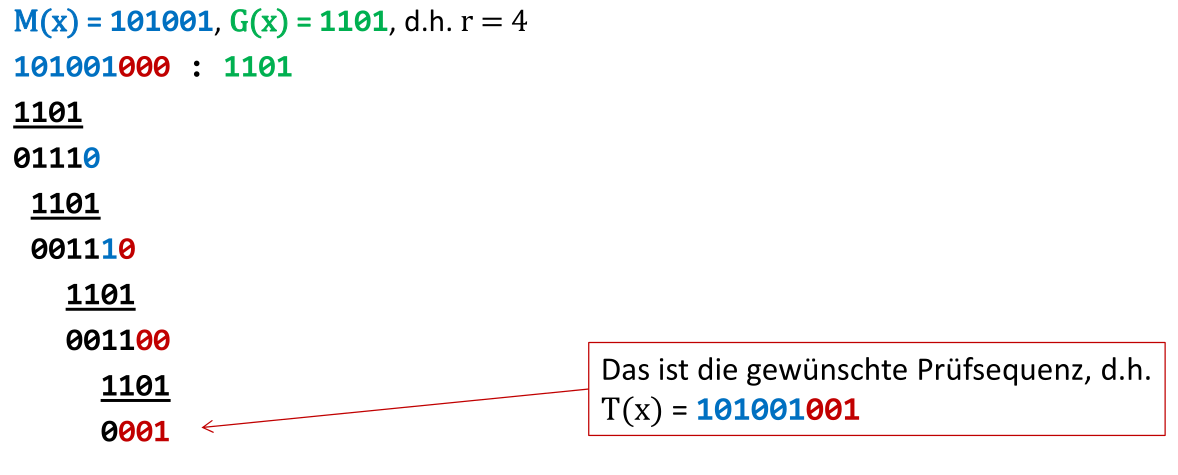
\includegraphics[width=7cm]{images/CRC/crc-gen.png} & 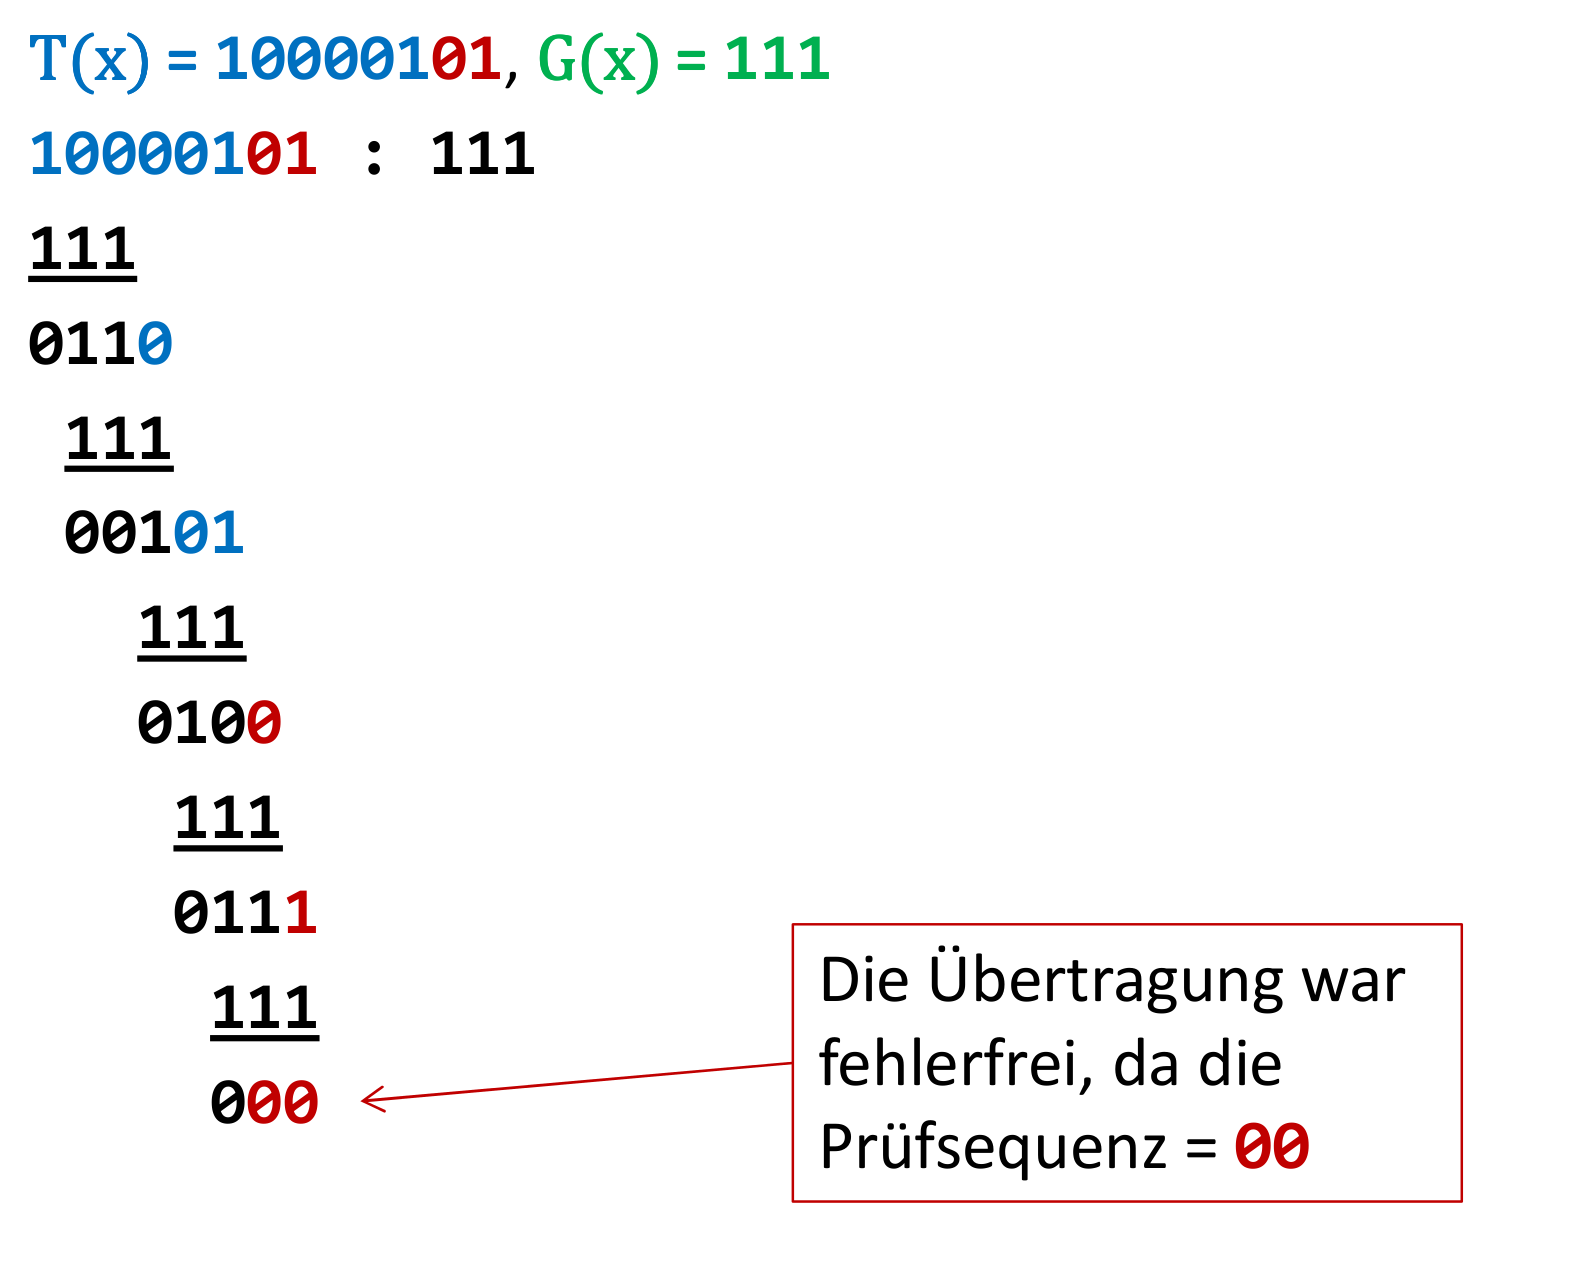
\includegraphics[width=7cm]{images/CRC/crc-enc.png}  \\ 
\end{tabular} 

\subsection{CRC in der Praxis}

\begin{tabular}{|c|c|c|}
\hline \textbf{Bezeichnung} & \textbf{Polynom} & \textbf{Verwendung} \\ 
\hline CRC-8-CCITT & 0x107 &  ATM, ISDN\\ 
\hline CRC-16-CCIT & 0x11021 & Bluetooth, SD-Card \\ 
\hline  CRC-16 & 0x18005  &  Modbus, USB\\
\hline  CRC-32 & 0x104C11DB7 & Ethernet, ZIP, Serial ATA, HDLC, PNG, usw. \\
\hline 
\end{tabular} 

\begin{itemize}
	\item Da das MSB des Polynoms immer 1 ist, wird dieses häufig bei der Beschreibung weggelassen, z.B. 0x8005 statt 0x18005 beim CRC-16
	\item Teilweise wird auch das LSB weggelassen, da dieses ebenfalls immer 1 ist	
\end{itemize}

\textbf{Softwareimplementationen}
\begin{itemize}
	\item Bit um Bit werden berechnet gemäss vorherigem Beispiel
	\item Werte werden vorberechnet und in einer Tabelle abgelegt	
\end{itemize}

\textbf{Hardwareimplementationen}
\begin{itemize}
	\item Linear rückgekoppeltes Schieberegister (Linear feedback shift register, LFSR)	
\end{itemize}

\textbf{Breite des Polynoms}
\begin{itemize}
	\item Die CRC-Polynome haben üblicherweise eine Breite von $(n \cdot 8 + 1)$, z.B. 9		
\end{itemize}

\textbf{Die XOR-Operation}
\begin{itemize}
	\item Eine XOR-Operation mit dem Remainder wird nur dann durchgeführt, wenn
	das oberste Bit des Remainders eine 1 ist, d.h. das oberste Bit des Resultats ist
	immer 0.
\end{itemize}
\newpage
\subsection{Implementation}
\subsubsection{Bit by Bit}
\begin{lstlisting}[style=C]
typedef uint8_t Crc;
enum {crcWidth = 8 * sizeof(Crc),
	crcTopBit = 1 << (crcWidth - 1)};
	
Crc crcSlow(const uint8_t message[], unsigned int nBytes)
{
	Crc remainder = 0;
	Crc crcPoly = 0x07;
	unsigned int byte;
	unsigned int bit;
	for (byte = 0; byte < nBytes; ++byte)
	{
		remainder ^= message[byte];
		for (bit = 8; bit > 0; --bit)
		{
			if (remainder & crcTopBit)
				remainder = (remainder << 1) ^ crcPoly;
			else
				remainder = (remainder << 1);
		}
	}
	return remainder;
}
\end{lstlisting}

\textbf{Nachteile}
\begin{itemize}
	\item Jedes Bit wird einzeln behandelt
	\begin{itemize}
		\item Pro Bit: AND, CMP, BNE, SHL, XOR
		\item Sehr aufwendig	
	\end{itemize}
	\item Langsam
\end{itemize}


\subsubsection{Tabelle}
\textbf{Ansatz}
\begin{itemize}
	\item Ein Byte hat 256 mögliche Werte, für jeden dieser Werte ist der dazugehörige CRC definiert. Dieser Wert liegt in einer Tabelle vor.
	\item Dadurch erzielt man eine Geschwindigkeitssteigerung um den Faktor 8	
\end{itemize}

\begin{lstlisting}[style=C]
typedef uint8_t Crc;
enum {crcWidth = 8 * sizeof(Crc),
	crcTopBit = 1 << (crcWidth - 1)};
	
Crc crcFast(const uint8_t message[], unsigned int nBytes)
{
	Crc remainder = 0;
	uint8_t data;
	unsigned int byte;
	for (byte = 0; byte < nBytes; ++byte)
	{
		data = message[byte] ^ remainder;
		remainder = crcTable[data];
	}
	return remainder;
}
\end{lstlisting}
